%\noindent {\bf Document editors:}~James Beacham, Brian Shuve \\
%\text{ \; }\\
%\text{ \; }\\

\noindent Particles in the Standard Model (SM) have lifetimes spanning an enormous range of magnitudes, from the $Z$ boson ($\tau\sim2\times10^{-25}$~s) through to the proton ($\tau\gtrsim10^{34}$ years) and electron (stable).

\begin{figure}[htb]
\centering
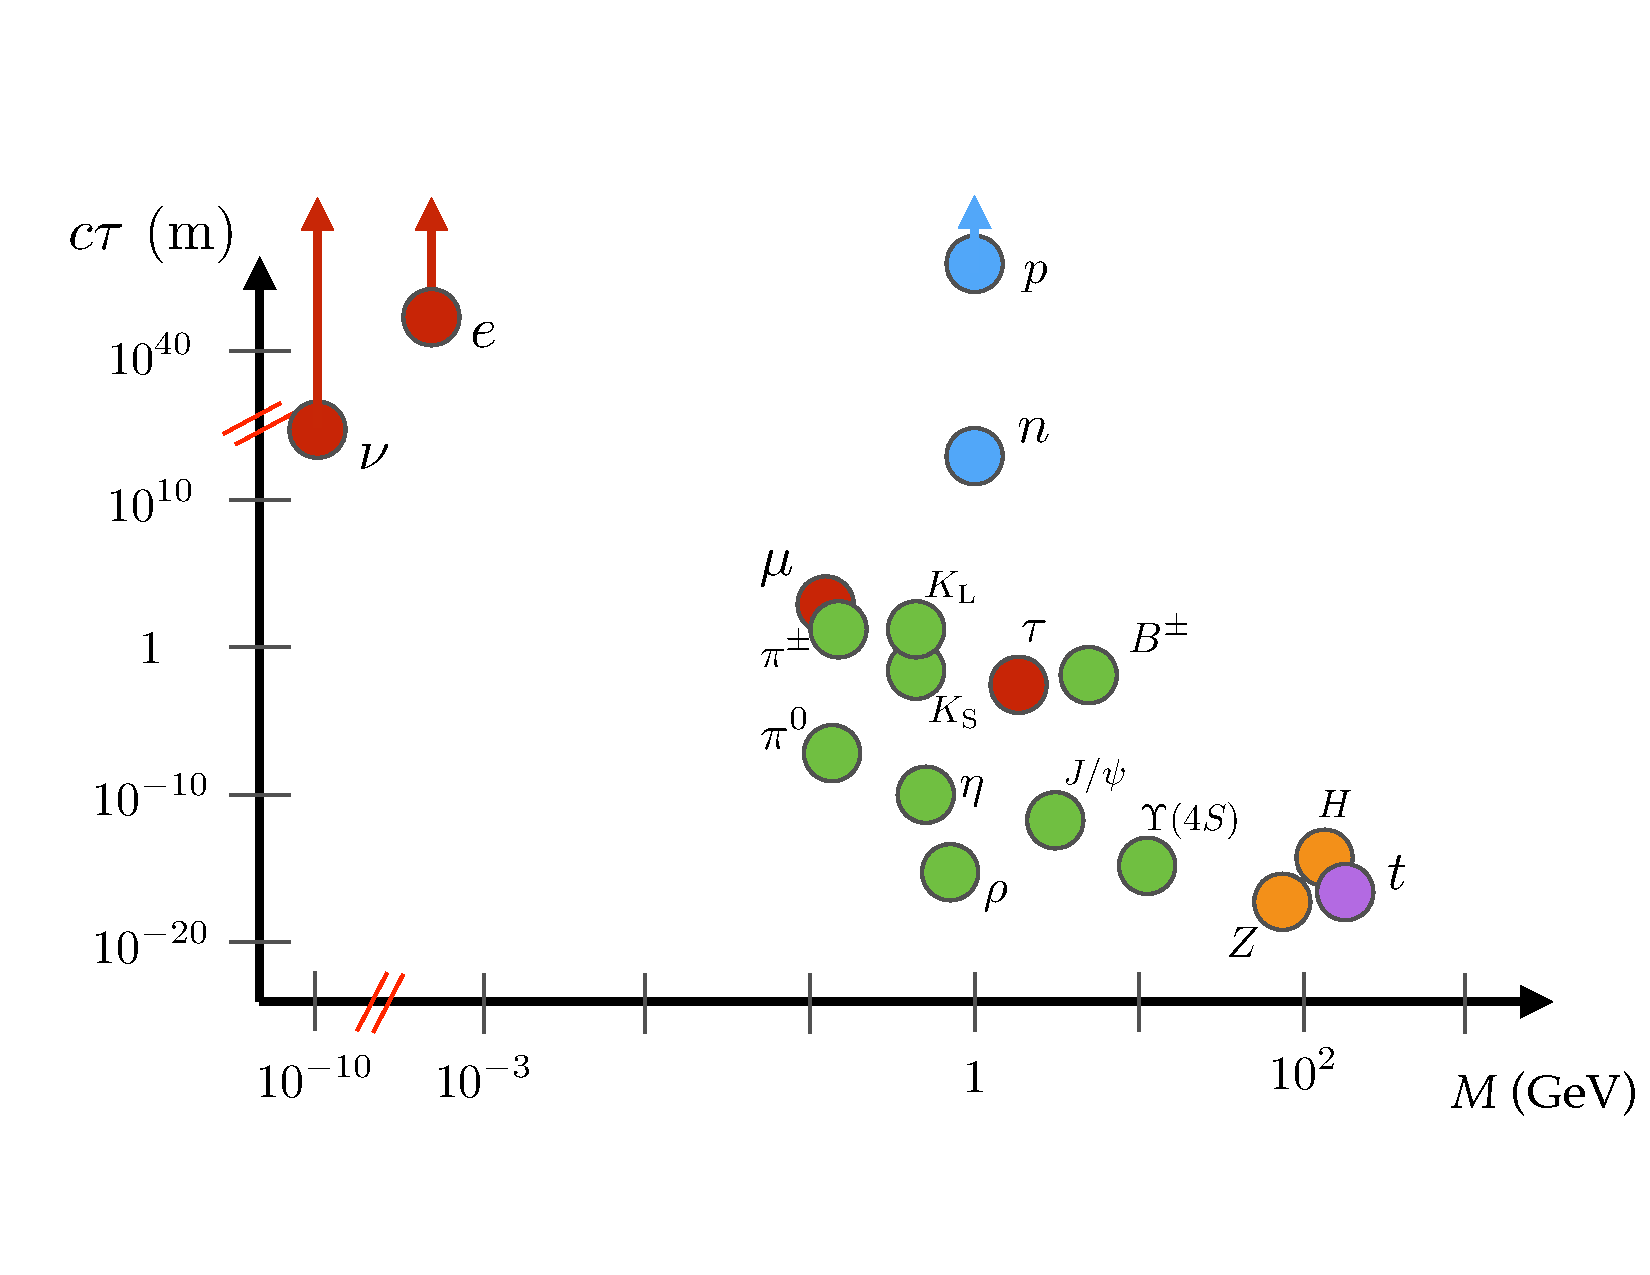
\includegraphics[width=0.9\textwidth]{plots/lifetime_plot.pdf}
\caption{Particle lifetime $c\tau$, expressed in meters, as a function of particle mass, expressed in GeV, for a variety of particles in the Standard Model.}
 \label{fig:SMLifetimes}
\end{figure}

Similarly, models beyond the SM (BSM) typically predict new particles with a variety of lifetimes \cite{massive-cite-dump}.
In particular, new weak-scale particles can easily have long lifetimes for several reasons, including approximate symmetries that stabilize the long-lived particle (LLP), small couplings between the LLP and lighter states, and suppressed phase space available for decays.
For particles moving close to the speed of light, this can lead to macroscopic, detectable displacements between the production and decay points of an unstable particle for $c\tau\gtrsim 10~\mu\mathrm{m}$. Recently, a comprehensive collection of the vast array of theoretical frameworks within which LLPs naturally arise has been assembled as part of the physics case document for the proposed MATHUSLA experiment~\cite{Curtin:2018mvb}. Because the focus of the current document is on the experimental signatures of LLPs and explicitly not the theories that predict them, the combination of the MATHUSLA physics case document (and the vast number of references therein) and the present document can be considered, together, a comprehensive view of the entirety of the possibilities, theoretical and experimental, for the potential discovery of LLPs produced at the interaction points of the LHC.

The experimental signatures of LLPs are varied and, by nature, are often very different from signals of SM processes.  For example, LLP signatures can include tracks with unusual ionization and propagation properties; small, localized deposits of energy inside of the calorimeters without associated tracks; stopped particles that decay out of time with collisions; displaced vertices in the inner detector or muon spectrometer; and disappearing, appearing, and kinked tracks.

\begin{figure}[htb]
\centering
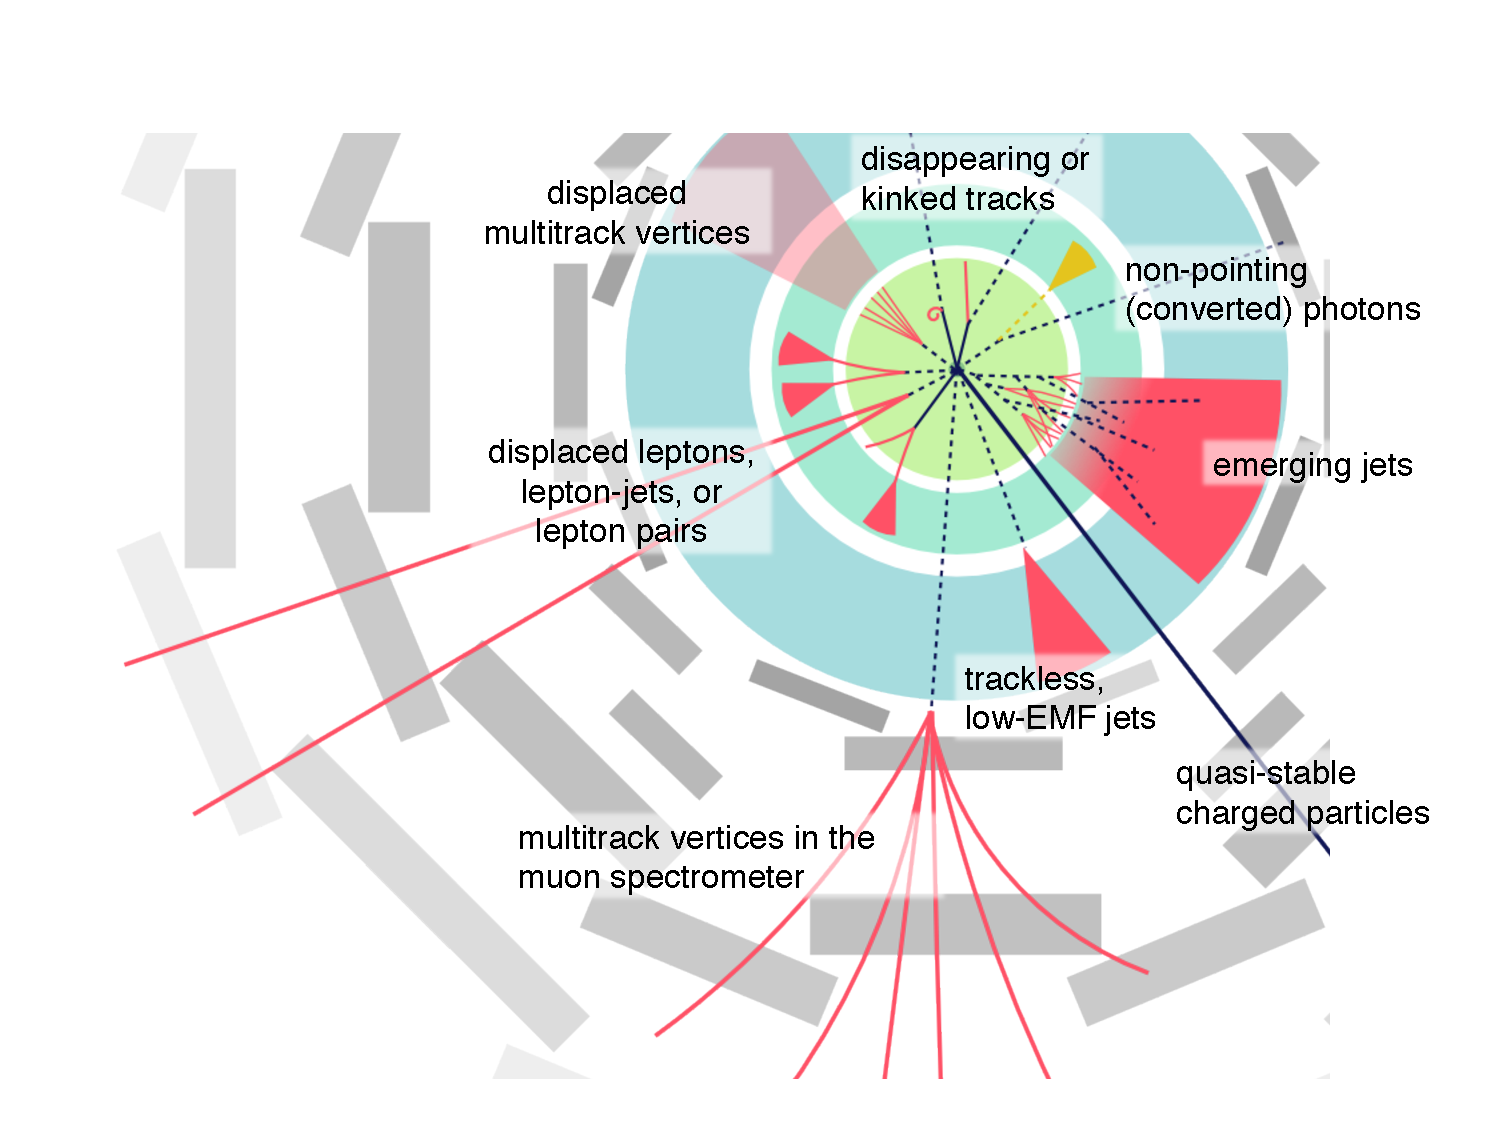
\includegraphics[width=0.9\textwidth]{plots/Heather_Russell_20170424_LLPs_Slide9.pdf}
\caption{Schematic of the variety of challenging, atypical experimental signatures that can result from BSM LLPs in the detectors at the LHC.  Shown is a cross-sectional plane in azimuthal angle, $\phi$, of a general purpose detector such as ATLAS or CMS.  From Ref.~\cite{Russell:2017AprilWorkshop}.}
 \label{fig:LLPSignaturesWheel}
\end{figure}

Because the long-lived particles of the SM have masses $\lesssim5$~GeV and have well-understood experimental signatures, the unusual signatures of BSM LLPs offer excellent prospects for the discovery of new physics at particle colliders.
At the same time, standard reconstruction algorithms may reject events or objects containing LLPs precisely because of their unusual nature, and dedicated searches are needed to uncover LLP signals.
These atypical signatures can also resemble noise, pile-up, or mis-reconstructed objects in the detector; due to the rarity of such mis-reconstructions, Monte Carlo (MC) simulations may not accurately model backgrounds for LLP searches, and dedicated methods are needed to do so.

Although small compared to the large number of searches for prompt decays of new particles, many searches for LLPs at the ATLAS, CMS, and LHCb experiments at the Large Hadron Collider (LHC)~\cite{another-massive-cite-dump} have already been performed; we refer the reader to Chapter \ref{sec:experimentcoverage} for descriptions of and references to these searches. Existing LLP searches have necessitated the development of novel methods for identifying signals of LLPs, and measuring and suppressing the relevant backgrounds.
Indeed, in several scenarios searches for LLPs have sensitivities that greatly exceed the search for similar, promptly decaying new particles (for example, this is true for directly produced staus in supersymmetry \cite{CMS-PAS-EXO-16-036}).
The excellent sensitivity of these searches, together with the lack of a definitive signal in any prompt channels at the LHC, have focused attention on other types of LLP signatures that are not currently covered.
These include low-mass LLPs that do not pass trigger or selection thresholds of current searches, high multiplicities of LLPs produced in dark-sector showers, or unusual LLP production and decay modes that are not covered by current methods.
Given the excellent  sensitivity of LHC detectors to LLPs, along with the potentially large production cross sections of LLPs and the enormous amount of data expected to be collected when the LHC switches to high-luminosity running in the 2020s, it is imperative that the space of LLP signatures be explored as thoroughly as possible to ensure that no signals are missed.
This is particularly important now, at the end of LHC Run 2, as decisions are currently being made about detector upgrades for Phase 2 of the LHC, and design decisions should be made to ensure that sensitivity to LLPs is retained or possibly improved through high-luminosity running.
Indeed, upgrades to the detectors may improve the sensitivity to LLPs compared to the conditions in Runs 1 and 2 of the LHC.

The growing theoretical and experimental interest in LLPs has been mirrored by an increased activity in proposals for LLP searches, new experimental analyses, and meetings to communicate results and discuss new ideas.
Workshops focused on LLPs at the University of Massachusetts, Amherst~\footnote{``LHC Searches for Long-Lived BSM Particles: Theory Meets Experiment'',~\url{https://www.physics.umass.edu/acfi/seminars-and-workshops/lhc-searches-for-long-lived-bsm\%2Dparticles-theory-meets-experiment}} in November of 2015; Fermilab; and KITP (UCSB)~\footnote{``Experimental Challenges for the LHC Run II'',~\url{http://online.kitp.ucsb.edu/online/experlhc16/}} in May of 2016, among others, highlighted the need for a community-wide effort to map the current space of both theoretical models for LLPs and the atypical experimental signatures that could be evidence of LLPs, assess the coverage of current experimental methods to these models, and identify areas where new searches are required.
Additionally, the work presented in these meetings highlighted the importance of presenting the results of experimental searches in a manner that allows for their application to different models, and generated new ideas for designing analyses with the goal of minimizing model dependence.
Such largely model-independent presentation makes current searches more powerful by increasing their applicability to new scenarios, while reducing redundancies in searches and ensuring that gaps in coverage are identified and addressed.
This task extends beyond the purview of any particular theoretical model or experiment, and requires an effort across collaborations to address the needs of the LLP community and illuminate a path forward.

This flurry of activity eventually coalesced in the establishment of a more central and regular platform --- the LHC LLP Community --- for experimentalists at the LHC and those in the theoretical and phenomenological communities to exchange ideas about LLP searches to ensure the full discovery potential of the LHC.
This began with a mini-workshop at CERN in May of 2016~\footnote{``LHC Long-Lived Particle Mini-Workshop'',~\url{https://indico.cern.ch/e/LHC_LLP_2016}} and has continued with workshops in April of 2017 at CERN~\footnote{``Searches for long-lived particles at the LHC: First workshop of the LHC LLP Community'',~\url{https://indico.cern.ch/e/LHC_LLP_April_2017}}, October of 2017 at ICTP Trieste~\footnote{``Searches for long-lived particles at the LHC: Second workshop of the LHC LLP Community'',~\url{https://indico.cern.ch/e/LHC_LLP_October_2017}}, and May of 2018 again at CERN~\footnote{``Searching for long-lived particles at the LHC: Third workshop of the LHC LLP Community'',~\url{https://indico.cern.ch/e/LHC_LLP_May_2018}}.

This is the work undertaken by the LHC LLP Community and presented in this document.
Based on the most pressing needs identified by the community, we organize the work of this initiative into a few key realms:
%
\begin{itemize}

\item {\bf Simplified models:}~We seek to identify a minimal (but expandable) set of simplified models that capture, with a very limited number of free parameters, the most important LLP signatures motivated by theory and accessible at the LHC.
The simplified models approach has been successfully applied to models such as supersymmetry (SUSY) and dark matter, and proposals exist for LLP simplified models in particular contexts.
We aim to provide a basis of models that serves as a focal point for the other studies performed by the community, as well as a library that can be used in simulating LLP signal events, to allow for a common grammar to better understand how current and future searches cover LLP signature space.

\item {\bf Experimental coverage:}~In spite of the many successful LLP searches undertaken by the ATLAS, CMS, and LHCb experiments, there remains a need for a systematic study of the complementary coverage of LLP searches to the parameter spaces of LLP models.
Having developed a simplified model basis, we provide a comprehensive overview of the sensitivity of existing searches, highlighting gaps in coverage and high-priority searches to be undertaken in the future.

\item {\bf Backgrounds to LLP searches:}~We provide a summary and analysis of backgrounds for LLP signals at the LHC, sources of which can be rare, unexpected, and largely irrelevant for searches for prompt BSM particles, and thus not fully well understood.
We assemble the collected knowledge and experience of backgrounds to prior searches with the intention of providing insight into the opportunities and challenges of searching for LLP signatures.

\item {\bf Upgrades and triggering strategies:}~We discuss the prospects for LLP searches with upgraded detectors for Phase 2 of LHC running, with a focus on how upgrades can offer new sensitivity to LLPs as well as mitigate the effects of pile-up. New opportunities for improving sensitivity of triggers and searches to LLPs are present for each planned upgrade beginning with Run 3.
This is tied to the crucial question of triggers for LLPs; we discuss the performance of current triggers for LLPs, as well as the effects of future upgrades to the trigger system.
Most importantly, we identify a few concrete upgrade studies that should be performed by the experiments that are of prime importance to the community.

\item {\bf Reinterpretation of LLP searches:}~Due to the non-standard nature of the objects used in analyses, LLP searches are notoriously hard to reinterpret for models beyond those considered by the experimental collaborations.
Designing searches and presenting search results in a way that is broadly applicable to current and yet-to-be-developed LLP models is crucial to the impact and legacy of the LLP search program.
We discuss the reinterpretation of the LLP searches by means of concrete examples to illustrate specific challenges and, based on the lessons learned from this procedure, we provide recommendations on the presentation of LLP experimental search results.

\item {\bf Dark showers:}~Current LLP search strategies have limited sensitivity to models where the LLPs are very soft, highly collimated, and come in large multiplicities, as can occur in models of dark-sector showers.
We report on recent progress in theoretically parameterizing the space of dark-shower models and signatures, as well as experimental searches to uncover these signals.
%We also discuss other frontiers in LLP searches where more research and development is needed to ensure comprehensive coverage.

\end{itemize}
%
Finally, we provide information about current and proposed experiments to search for LLPs at the LHC via dedicated detectors.
These include the MoEDAL monopole search, the milliQan milli-charged particle experiment, the MATHUSLA surface detector for ultra-LLPs, the CODEX-b proposal for a new detector near LHCb, and the FASER proposal for a long, narrow detector located in the forward direction well downstream one of the collision points.

This is the first report of the LHC LLP Community initiative, and is expected to be followed by future reports as our collective understanding of these signatures as a means of discovering new physics at the LHC evolves.
